% \ifx\handouts\undefined
 \documentclass{beamer}
% \else
%\documentclass[xcolor=svgnames,handout]{beamer}
%\fi

\mode<presentation>
{
\useoutertheme{miniframes}
\setbeamercovered{transparent}
}

\setbeamertemplate{footline}[frame number]

\usepackage{babel}
\usepackage[utf8]{inputenc}
\usepackage{times}
\usepackage[T1]{fontenc}
\usepackage{moreverb}
\newcommand{\code}[1]{\texttt{#1}}
\let\overbatim\verbatim
\let\endoverbatim\endverbatim
\newenvironment{vcode}%
{\bgroup\baselineskip=0.8\baselineskip\overbatim}%
{\endoverbatim\egroup}


\newcounter{demo}
\newcommand{\Demo}{\stepcounter{demo}\frametitle{Demo \arabic{demo}}}

\title{R: language and basic data management} 

%HARJUTA JA VÕTA AEGA - PEAD HAKKAMA SAAMA 45 MINUTIGA!

%DEMODE ASEMEL PANE NÄITED - INPUT-OUTPUT SLAIDIDIELE!
\author{Krista~Fischer}

\date[Tartu 2019] % (optional)
{Statistical Practice in Epidemiology, Tartu, 2019 \\ (initial slides by P. Dalgaard)}


% If you wish to uncover everything in a step-wise fashion, uncomment
% the following command: 

%\beamerdefaultoverlayspecification{<+->}


\begin{document}

\begin{frame}
  \titlepage
\end{frame}

\section{Basics}

\begin{frame}
  \frametitle{Language}
  \begin{itemize}
  \item R is a programming language -- also on the command line
  \item (This means that there are \emph{syntax rules})
  \end{itemize}
On the command line (or a line in a script) one could:
  \begin{itemize}
  \item Print an object by typing its name
  \item Evaluate an expression 
  \item Call a function, giving the arguments in parentheses -- possibly empty
  \item Notice \code{objects} vs. \code{objects()}
  \end{itemize}
\end{frame}


\begin{frame}
  \frametitle{R expressions}
\texttt{\alert<6>{\alert<2>{x} <-} \alert<5>{rnorm(\alert<3>{10}, mean=\alert<3>{20}, 
 sd=\alert<3>{5})}\\
\alert<6>{\alert<2>{m} <-} \alert<5>{mean(\alert<2>{x})}\\
\alert<5>{sum((\alert<2>{x} \alert<4>{-} \alert<2>{m})\alert<4>{\textasciicircum}\alert<3>{2})}
}\\
\pause
  \begin{itemize}
  \item Object \alert<2>{names}
  \item Explicit \alert<3>{constants}
  \item Arithmetic \alert<4>{operators}
  \item \alert<5>{Function calls}
  \item \alert<6>{Assignment} of results to names
  \end{itemize}
\end{frame}

\section{Objects in R}

\begin{frame}
  \frametitle{Objects}
  \begin{itemize}
  \item The simplest object type is \emph{vector}
  \item Modes: numeric,  character,  factor, \ldots
  \item Operations are vectorized: you can add entire vectors with
    \code{a + b}
  \item Recycling of objects: If the lengths don't match, the shorter
    vector is reused 
  \end{itemize}
\end{frame}


%\addtocounter{framenumber}{-1} %% workaround for beamer buglet
\begin{frame}[fragile]
\frametitle{Example (numeric vectors)}
\begin{vcode}
> a <- c(2, 8, 3, 1, 0, 7)
> b <- c(3, 4, 1, 4, 5, 2)
> a+b
[1]  5 12  4  5  5  9
> mean(a)
[1] 3.5
> m <- mean(a)
> m
[1] 3.5
> a - m # notice recycling
[1] -1.5  4.5 -0.5 -2.5 -3.5  3.5

> z <- c(1, 2, 3)
> a - z   #recycling!
[1]  1  6  0  0 -2  4
\end{vcode}
\end{frame}


\begin{frame}[fragile]
  \frametitle{Factors}
  \begin{itemize}
%  \item The elements of character vectors are text strings that do not have any numeric value.  
  \item \alert{Factors} are used to describe groupings -- these are just integer codes plus a set of names, as labels for
    the \emph{levels}
  \item In model specifications, a factor variable is treated as a classification
    rather than as a quantitative variable
  \end{itemize}
 Example: 
\begin{vcode}
> x<-c(1,3,3,2,1,3,1)
> fx<-factor(x,labels=c("bad","average","good"))

> fx
[1] bad     good    good    average bad     good    bad    

 > levels(fx)
[1] "bad"     "average" "good"       
\end{vcode}     
\end{frame}
%  \item Notice that there is a slightly confusing use of \code{levels} and
  %  \code{labels} arguments.
 % \item \code{levels} are the value codes \emph{on input}
  %\item \code{labels} are the value codes \emph{on output} (and become
   % the levels of the resulting factor)


\begin{frame}
  \frametitle{Lists}
  \begin{itemize}
  \item Lists are vectors where the elements can have different types -- thus collections of any elements, gathered into one object
  \item Functions often return lists
  \item \code{lst <- list(A=rnorm(5), B="hello")}
  \item Special indexing:
  \item \code{lst\$A}
  \item \code{lst[[1]]} first element (NB: double brackets)
  \item \alert{Data frames} are special type of lists
  \end{itemize}
\end{frame}

\begin{frame}[fragile]
  \frametitle{Matrices}
  \begin{itemize}
  \item A \alert{matrix} is a rectangular collection of data. All columns of a matrix should be of the same type.  
\begin{vcode}
> A<-matrix(c(1,4,2,6,7,8),nrow=3,ncol=2,
                                 byrow=T)
> A
     [,1] [,2]
[1,]    1    4
[2,]    2    6
[3,]    7    8

\end{vcode}
  \item One can also construct a matrix from its
    columns using \code{cbind}, whereas joining two matrices with equal no of columns (with the same column names) can be done using \code{rbind}.
  \end{itemize}
\end{frame}

\begin{frame}[fragile]
  \frametitle{Data frames}
  \begin{itemize}
\item Usually a dataset in R is stored in a form of a \alert{data frame}. 
\item While reading in data from text files (using \code{read.table(), read.csv()}), a data frame is created.
\item A data frame is similar to a matrix, but can have columns (variables) of different types.
\item A variable can be extracted using \code{dataframe\$variable} (as data frames are lists) 
\begin{vcode}
> D<- data.frame(a=c(8,3,5),b=c("X","Z","Y"))
> D
  a b
1 8 X
2 3 Z
3 5 Y
> D$a
[1] 8 3 5
\end{vcode}
  \end{itemize}
\end{frame}

\begin{frame}[fragile]
  \frametitle{Matrices or data frames?}
  \begin{itemize}
\item A (numeric or character) matrix can be converted to a data frame and vice versa (with \code{as.data.frame(A)} and \code{as.matrix(B)}).
\item  Most R functions for statistical analysis work with data frames, but in some cases it is useful to have a matrix (incl the occasions where you want to use some matrix algebra).  
\item If you need more dimensions than two, there is also \code{array}. 
  \end{itemize}
\end{frame}


\section{Data frames and data manipulation}
\begin{frame}[fragile] 
\frametitle{How to access variables in the data frame?} 
Different ways to tell R to use variable X from data frame D: 
\begin{itemize}
\item  As mentioned, you can use the \verb!dataframe$variable! notation
\begin{vcode}
summary(D$X)
\end{vcode}
\item Use the \code{with} function
\begin{vcode}
with(D, summary(X))
\end{vcode}
\item Use the \code{data} argument (does not works for all functions)
\begin{vcode}
lm(Y~X, data=D)
\end{vcode}
\item  Attach the dataframe -- \alert{DISCOURAGED!}\\ {\small (seems a convenient solution, but can actually make things more complicated, as it creates a temporary copy of the dataset)}
\begin{vcode}
attach(D)
summary(X)
detach()
\end{vcode}
\end{itemize}
\end{frame}


\begin{frame}[fragile]
\frametitle{Data manipulation}
To create a new variable \code{bmi} in the existing data frame \code{students}, use either of the two:
\begin{vcode}
students$bmi <- 
       with(students, weight/(height/100)^2)
students <-
     transform(students, bmi=weight/(height/100)^2)
\end{vcode}
(notice: you need an assignment, to save the transformed object)
\mbox{  }\\[0.3cm]
%{\small 
%whereas
%\begin{vcode}
%with(students,  bmi <- weight/(height/100)^2)
%\end{vcode}
%creates the variable \code{bmi} in the global environment (not in the data frame). 
 %}

\end{frame}

%\section{Indexing}
\begin{frame}
  \frametitle{Indexing -- extracting elements from objects}
 \alert{{\large Square brackets \code{[} \code{]} are used for indexing!}}\\[0.2cm]
 % R has several useful indexing mechanisms of form \code{x[cond]} for vectors, \code{x[row.cond, col.cond]} for matrices or data %frames. For instance:
 Examples:
  \begin{itemize}
   \item Elements of vectors: \code{a[5]} (5th element);  \code{a[5:7]} (5th to 7th elements);  \code{a[-6]} (all elements except the 6th)
  \item Logical index:  \code{a[a<3]},  \code{a[b>2]} , \code{a[is.na(b)]} (elements of \code{a} corresponding to missing values of \code{b})
\item In a data frame or matrix -- two dimensions, two indexes: \\ \code{students[5, 7]},  
\code{students[1:10, c(2,5)]}, \\  \code{students[1, ], students[ ,3]  (entire row/column)}
\end{itemize}
\end{frame}

%\addtocounter{framenumber}{-1} %% workaround for beamer buglet
\begin{frame}[fragile]
  \frametitle{Examples of indexing} 
  \begin{vcode}
>  x<- c(2,7,3,1,5,9,0)
> x[c(1,5,7)]
[1] 2 5 0
> x[x<3]
[1] 2 1 0

> NMRimp[1:2,1:4]    #quick look at a large data
  sample.id XXL.VLDL.P XXL.VLDL.L XXL.VLDL.PL 
1    V18566   1.46e-04     0.0313     0.00331  
2    V36115   9.00e-05     0.0195     0.00178    

> fgsa[is.na(fgsa$height),"age"]  
  [1] 18 69 52 41 52 44 73 28 66 20 73 63 26 
# ages of those with missing height

# equivalent: fgsa$age[is.na(fgsa$height)]   
\end{vcode}
\end{frame}

%\addtocounter{framenumber}{-1} %% workaround for beamer buglet
%\begin{frame}[fragile]
%  \frametitle{Conditional assignment: \texttt{ifelse}}
%  \begin{itemize}
%  \item Syntax: \code{ifelse(expression,A,B)} \\
%Expression (with values TRUE or FALSE) is a vector, A and B are constants or vectors of the same length.
% \end{itemize}
%Examples: %\Demo
%\begin{vcode}
%> x<-c(1,2,7,3,NA)
%> ifelse(x<3,1,2)
%[1]  1  1  2  2 NA
%> ifelse(is.na(x),0,x) #replace missing values by 0 
%[1] 1 2 7 3 0
%>  y<-c(3,6,1,7,8);  z<-c(0,1,0,2,1)
%>  ifelse(z==0,x,y)
%[1] 1 6 7 7 8
%>  ifelse(is.na(x),0,ifelse(x>3,3,x)) 
%[1] 1 2 3 3 0
%\end{vcode}
%\end{frame}

\begin{frame}[fragile]
  \frametitle{Naming}
  \begin{itemize}
  \item Elements of vectors, rows and columns of matrices and data frames can have names
\begin{vcode}
> x <- c(boys=1.2, girls=1.1)
> x
 boys girls 
  1.2   1.1 
> x["boys"]
boys 
 1.2
> D[,"a"]  # works for matrices and data frames
[1] 8 3 5
\end{vcode}
  \item You can extract and set names with \code{names(x)}; for matrices and data frames also \code{colnames(x)} and \code{rownames(x)};
 \end{itemize}
\end{frame}


\begin{frame}[fragile]
  \frametitle{Classes, generic functions}
  \begin{itemize}
  \item R objects have \emph{classes} 
  \item Functions can behave differently depending on the class of an
    object 
  \item E.g. \code{summary(x)} or \code{print(x)} does different
    things if \code{x} is numeric, a factor, or a linear model fit
  \end{itemize}
\begin{vcode}
  > summary(x)  # a numeric vector
   Min. 1st Qu.  Median    Mean 3rd Qu.    Max. 
      1       1       2       2       3       3 
> summary(fx) # a factor
    bad average    good 
      3       1       3 
\end{vcode}
\end{frame}

\section{Functions}
\begin{frame} 
  \frametitle{Function calls}
 \alert{{\large Round brackets \code{(} \code{)} are used for function calls!}}\\[0.2cm]
  Lots of things you do with R involve calling functions (you have seen that already!).\\
  For instance
  \begin{center}
    \large
    \texttt{\alert<2>{mean}(\alert<3>{x}, \alert<4>{na.rm=\alert<3>{TRUE}})}
  \end{center}
  The important parts of this are
  \pause
\begin{itemize}
\item The \alert<2>{name} of the function
\item \alert<3>{Arguments}: input to the function
 \item Sometimes, we have \alert<4>{named arguments}
\end{itemize}
\end{frame}

\begin{frame}
  \frametitle{Function arguments}
Examples:
  \begin{center}
    \large
\texttt{
rnorm(\alert<3>{10}, \alert<6>{mean=}\alert<2>{m}, 
    \alert<6>{sd=}\alert<2>{s})\\
hist(\alert<2>{x}, \alert<6>{main=}\alert<3>{"My histogram"})\\
mean(\alert<4>{log(x + 1)})}
  \end{center}
Items which may appear as arguments:
  \begin{itemize}
  \item \alert<2>{Names} of R objects
  \item Explicit \alert<3>{constants}
  \item \alert<4>{Return values} from another function call or expression
  \item Some arguments have their \emph{default values}. 
\item 
Use \code{help(\textit{function})} or  \code{args(\textit{function})} to see the arguments (and their order and default values) that can be given to any function. 
\item Quite often -- first argument is not named, but the others are named
 % \item Keyword matching: \code{t.test(x \textasciitilde{} g, mu=2, alternative="less")}
 % \item Partial matching: \code{t.test(x \textasciitilde{} g, mu=2, alt="l")}
  \end{itemize}
\end{frame}

\begin{frame}[fragile]
\frametitle{Example}
From R-help (\code{help(t.test)}):
\begin{vcode}
t.test(x, y = NULL,
   alternative = c("two.sided","less","greater"),
   mu = 0, paired = FALSE, var.equal = FALSE,
   conf.level = 0.95, ...)
\end{vcode}
  \begin{itemize}
\item The first argument (x) does not have a default -- you have to provide some data!
\item The other arguments can be modified, if you need to.
  \end{itemize}
  \end{frame}

\begin{frame}[fragile]
\frametitle{Example (cont.)}
The following lines of code are equivalent:
\begin{vcode}
t.test(a, b,  alternative="less", paired=TRUE)
t.test(a, b, paired=TRUE, alt="less")

t.test(a, b, p=T, a="l")   #not a good style!
\end{vcode}
Order does not matter for named arguments! \\ 
Partial keyword matching is possible (``alternative" or ``alt'' or ``a") (partial matching is possible) 

\alert{For a readable code, the use of explicit argument names is highly recommended!}
\end{frame}

\section{Graphics}
\begin{frame}[fragile]
\frametitle{Basic graphics}
The \code{plot()} function is a generic function, producing different plots for different types of arguments. For instance, \code{plot(x) } produces:
\begin{itemize}
\item a plot of observation index against the observations, when \code{x} is a numeric variable %(witn numeric \code{x} and \code{y}, \code{plot(x,y)} produces a scatterplot)
\item a bar plot of category frequencies, when \code{x} is a factor variable
\item a time series plot (interconnected observations) when \code{x} is a time series
\item a set of diagnostic plots, when  \code{x} is a fitted regression model
\item Similarly, the \code{plot(x,y)} produces a scatter plot, when \code{x} is a numeric variable
and a bar plot of category frequencies, when \code{x} is a factor variable
\end{itemize}
\end{frame}

\begin{frame}[fragile]
\frametitle{Some simple plots:}
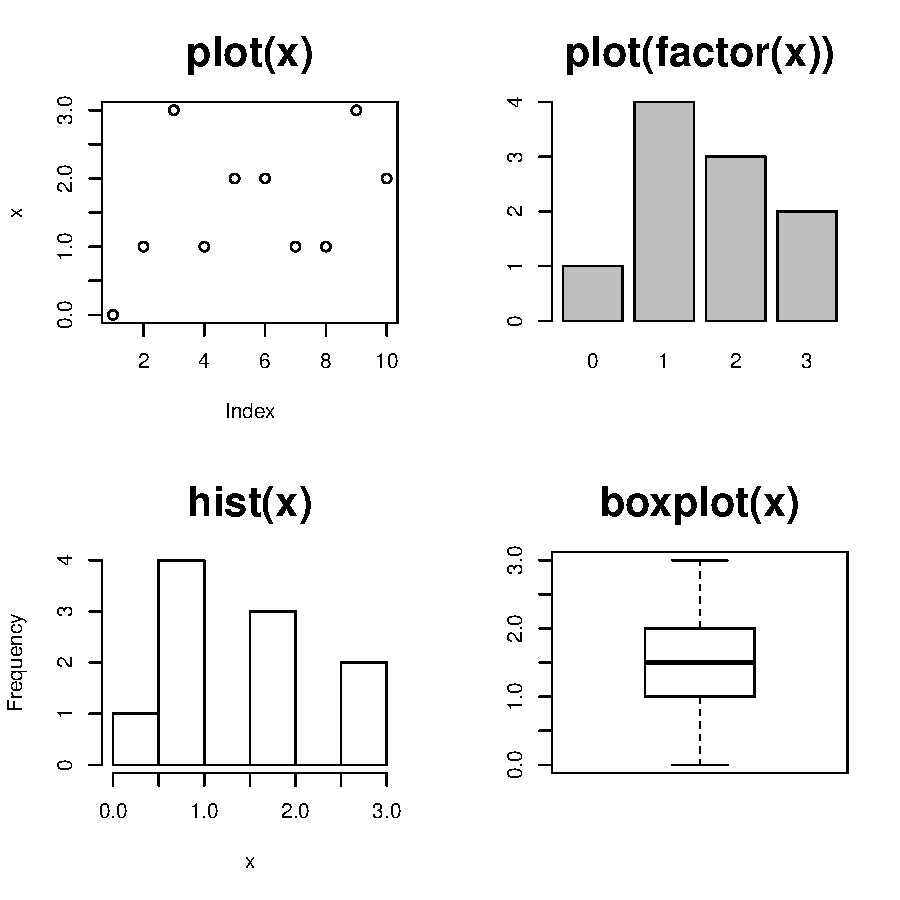
\includegraphics[width=0.75\textwidth]{spe_intro_plots}
\end{frame}

%\addtocounter{framenumber}{-1} %% workaround for beamer buglet


\section{The workspace}

\begin{frame}{}
  \frametitle{The workspace}
  \begin{itemize}
  \item The \emph{global environment} contains R objects created on the
    command line. 
  \item There is an additional \emph{search path} of loaded packages
    and attached data frames.
  \item When you request an object by name, R looks first in the
    global environment, and if it doesn't find it there, it continues
    along the search path.
  \item The search path is maintained by \code{library()},
    \code{attach()}, and \code{detach()}
  \item Notice that objects in the global environment may mask objects
    in packages and attached data frames
  \end{itemize}
\end{frame}

\section{Additional topics}
\begin{frame}
  \frametitle{More on factors: the \code{cut} Function}
  \begin{itemize}
  \item The \code{cut} function converts a numerical variable into groups
  (a factor variable)  according to a set of break points
  \item The intervals are left-open, right-closed by
    default (\code{right=FALSE} changes that)
  \item \dots and that the lowest endpoint is \emph{not} included by
    default (set \code{include.lowest=TRUE} if it bothers you)
  \end{itemize}
\end{frame}

%\addtocounter{framenumber}{-1} %% workaround for beamer buglet
\begin{frame}[fragile]
Example
\begin{vcode}
> age <- c(35,20,21,50,46,23,30)
> agegr<-cut(age, c(20,30,40,50))
> table(agegr)  
agegr      # the 20-year old is not included!
(20,30] (30,40] (40,50] 
      3       1       2 
> agegr<-cut(age, c(20,30,40,50),right=FALSE)
> table(agegr)
agegr    # the 50-year old is not included!
[20,30) [30,40) [40,50) 
      3       2       1 
> agegr<-cut(age, c(20,30,40,50),
+                           include.lowest=TRUE)
> table(agegr)
agegr
[20,30] (30,40] (40,50] 
4       1       2 \end{vcode}
\end{frame}

%\addtocounter{framenumber}{-1} %% workaround for beamer buglet
\begin{frame}[fragile]
  \frametitle{Working with Dates}
  \begin{itemize}
  \item Dates are usually read as character or factor variables
    \pause
  \item Use the \code{as.Date} function to convert them to objects of
    class \code{"Date"}
    \pause
  \item If data are not in the default format (YYYY-MM-DD) you need to
    supply a format specification

    \begin{vcode}
> as.Date("11/3-1959",format="%d/%m-%Y")
[1] "1959-03-11"
    \end{vcode}
    \pause
  \item You can calculate differences between \code{Date} objects. The
    result is an object of class  \code{"difftime"}. To get the number
    of days between two dates, use

    \begin{vcode}
> as.numeric(as.Date("2017-6-1")-
             as.Date("1959-3-11"),"days")
[1] 17607
    \end{vcode}
  \end{itemize}
\end{frame}


\begin{frame}[fragile]
\frametitle{Creating your own functions}
%\Demo
A very simple example: 
\begin{vcode}
logit <- function(p)  log(p/(1-p))
\end{vcode}
The function \code{logit} requires one argument $p$ and produces the logit of $p$. Try  
\code{logit(0.5)}, or \code{logit(0.25)}, \ldots \\[0.3cm]
More complex (but still simple):
\begin{vcode}
simpsum <- function(x, dec=5) {
m <- mean(x, na.rm=TRUE)
s  <- sd(x, na.rm=TRUE)
 round(c(mean=m,sd=s), dec) } 
\end{vcode}
The function \code{simpsum} requires one argument $x$, but the second argument \code{dec} (no of decimal points in the output) has a default value 5. Try \code{simpsum(a)}, or \code{simpsum(a,dec=2)}.
\end{frame}


\end{document}